%!TEX root = ../template.tex
%%%%%%%%%%%%%%%%%%%%%%%%%%%%%%%%%%%%%%%%%%%%%%%%%%%%%%%%%%%%%%%%%%%
%% chapter1.tex
%% NOVA thesis document file
%%
%% Chapter with introduction
%%%%%%%%%%%%%%%%%%%%%%%%%%%%%%%%%%%%%%%%%%%%%%%%%%%%%%%%%%%%%%%%%%%
\typeout{NT FILE chapter8.tex}%

\chapter{Evaluation and Results}
\label{chap:results_eval}

Fazer a intro do capitulo 

\section{Objectives and Evaluation Method}

The evaluation was an important and necessary step to understand how well the system supports its intended users in practice. Beyond testing the design choices, it was important to verify whether the tool could offer a smooth and intuitive experience, allow natural interaction when constructing proofs, and provide effective feedback that helps students progress in their learning. For this reason, the evaluation focused on three main objectives: the usability of the interface, the interactivity of proof construction, and the effectiveness of the feedback system.

To proceed with this evaluation, we followed the formative evaluation approach. Formative evaluation is a systematic process used to assess and improve the quality of software systems and tools during development. In educational computing, it is a powerful technique for creating high-quality educational software by providing feedback throughout the development process [https://doi.org/10.1080/08886504.1999.10782276]. This evaluation can be carried out in two ways: analytically, where usability specialists review the interface using their knowledge and rules without involving real users, or empirically, where the interface is tested by observing real users and collecting data from their actions.

The tests we conducted were empirical and carried out through online meetings with real users of different types (see [REF USER TYPES]). Each meeting began with a brief introduction to the tools and their functionality. This introduction was kept superficial, as we did not want users to memorize the procedures; we only wanted them to have a general understanding of what was possible with the tool. After the introduction, users were asked to complete a set of activities designed to evaluate the three objectives mentioned earlier. During the activities, users were encouraged to think aloud so that we could better understand their needs and follow their reasoning. While they completed the activities, we took notes on their actions and comments. Some activities were more restricted to cover specific objectives, while others allowed users greater freedom. Certain activities were timed to provide a quantitative measure of system performance. Users completed the activities on either computers or tablets, allowing us to test the tool in different environments. At the end of the sessions, users were asked to fill in a SUS questionnaire, which collected additional quantitative data.

\section{Participants}
For the tests we conducted, we tried to select users from all types. Unfortunately, we could not find Beginner students, that is, users who were just starting to learn \gls{ND} proofs, because the tests were conducted during the summer holidays and there were no students beginning this topic at that time. Instead, we tested with past students who had learned these proofs some years ago but did not remember much about them.

For the remaining user types, we were able to find participants. For the Intermediate and Experienced students, we tested students who had learned these exercises recently. For the Teacher group, we worked with a variety of teachers from NOVA University Lisbon, including some who are currently coordinating the Logic course where these exercises are taught, as well as others who had taught the course in previous editions. One of the teachers had also been a student who taught the practical classes in a previous edition.

Overall, the tests were conducted with 12 users: 3 Beginner students (all past students), 3 Intermediate students, 2 Experienced students, and 4 Teachers.

\section{Tasks}
To evaluate the users, we conducted two different activities. In both activities, users were asked to construct a proof for a given problem.

The first activity was more restricted: users had to follow the exact steps described in the instructions. The goal of this activity was to test the usability and interactivity of the tool by guiding users through important aspects of the proof (these aspects are detailed in the activity description). This activity was timed to provide an indication of how intuitive and easy to navigate the interface is, and how smoothly it supports constructing proofs. The activity also included a component to test the effectiveness of error and feedback messages, although this was not the main focus.

The second activity was more open and varied depending on the type of user. For students, they were asked to select a exercise and build the proof in their preferred way, without any time limits. The goal was to see if they could complete the full proof independently, using their knowledge of \gls{ND} proofs and the tool’s error and feedback system if they encountered difficulties. This allowed us to analyze how useful and effective the messages are and whether users could overcome difficulties with their help. For teachers, a similar open approach was used. They were asked to solve a problem without restrictions, but the focus was on intentionally making errors to test the variety, accuracy, and usefulness of the system’s feedback and error messages. In this case, the goal was not to see if teachers could complete the proof, but to evaluate the tool’s feedback system more thoroughly.

\subsection*{First Activity}
The goal of the first activity was to prove the tautology:
\[
\vdash (b \rightarrow c) \rightarrow ((a \wedge b) \rightarrow (a \wedge c))
\]

The activity was divided into the following tasks:

\begin{enumerate}
    \item \textbf{Apply the Introduction Rules.} 
    Users identified the main block containing the final conclusion and applied the $\to_I$ rule to that block, assigning it mark 1 and filling in the hypothesis. If unsure, they could hover over the rule or tap the ``?'' icon to see a tooltip preview. This process was repeated for the new hypothesis, assigning mark 2 to the second Implication Introduction. The focus of this task was to evaluate whether adding rules and assigning marks is intuitive, and whether the tooltip helps users complete the step.  
    \begin{center}
        \fbox{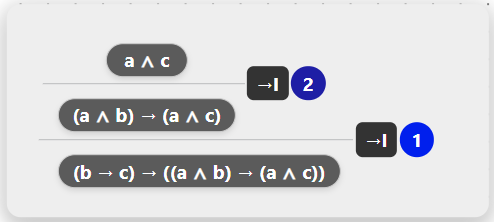
\includegraphics[width=0.5\textwidth]{Chapters/Figures/a1-task1.png}}
    \end{center}

    \item \textbf{Prove $a$.} 
    Users added a new tree, filled it with $a$, applied the $\land_{E_r}$ rule, and filled the new hypothesis with $a \land b$, assigning mark 2. They then validated the proof using ``Check proof.'' This task tested whether adding a new proof, assigning marks, and submitting the proof was intuitive.  
    \begin{center}
        \fbox{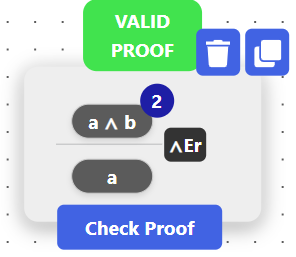
\includegraphics[width=0.35\textwidth]{Chapters/Figures/a1-task2.png}}
    \end{center}

    \item \textbf{Prove $c$.} 
    Users added another tree with $c$, applied the $\to_E$ rule, inserted $b$ in the first hypothesis and $b \to c$ in the second, and applied $\land_{E_l}$ to prove $b$ from $a \land b$, marking it with 2. They validated the proof after completion.  This task evaluated how intuitively users could enter formulas without the auxiliary keyboar in the proof.
    \begin{center}
        \fbox{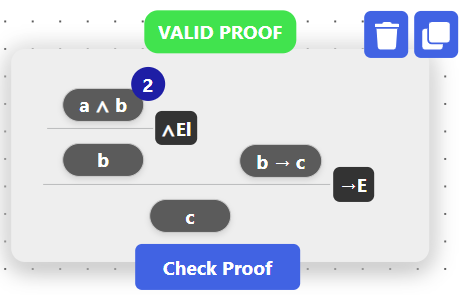
\includegraphics[width=0.45\textwidth]{Chapters/Figures/a1-task3.png}}
    \end{center}

    \item \textbf{Connect All Trees.} 
    Users applied the $\land_I$ rule to the first tree’s hypothesis, dragged the tree concluding $a$ to the right hypothesis and $c$ to the left, and checked the full proof. Some manipulations were intentionally challenging to test error handling and block movement. This step evaluated the interactivity of the system and how users manage moving proof blocks.  
    \begin{center}
        \fbox{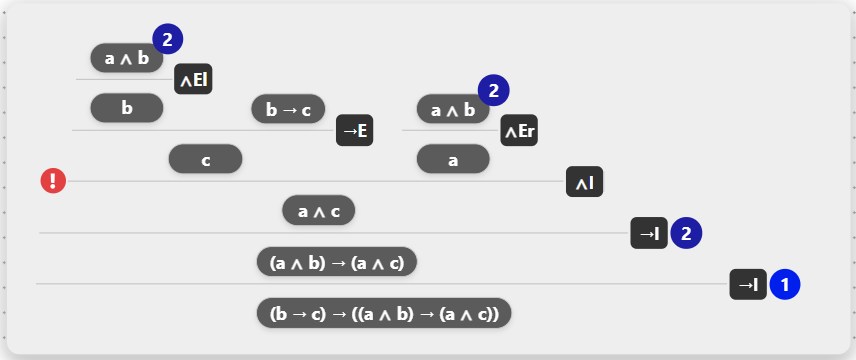
\includegraphics[width=0.65\textwidth]{Chapters/Figures/a1-task4.png}}
    \end{center}

    \item \textbf{Correct the Errors.} 
    Users corrected remaining errors and clicked ``Check proof'' until the message ``Problem solved'' appeared. They could freely move or extract blocks as needed.  
    The final task assessed the usability of block manipulation and the effectiveness of error and feedback messages.  
    \begin{center}
        \fbox{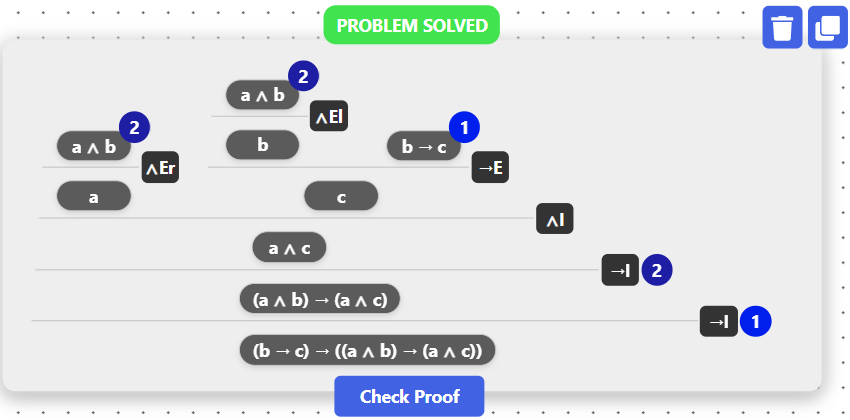
\includegraphics[width=0.65\textwidth]{Chapters/Figures/a1-task5.png}}
    \end{center}
\end{enumerate}

\subsection*{Second Activity}

\subsubsection*{Student Version}
In this task, students were asked to complete a proof independently. After becoming familiar with the basic steps in the first activity, they were free to decide how to proceed. Students were asked to prove one of the following:

\begin{center}
$\{(a \lor b) \land (a \lor c)\} \vdash a \lor (b \land c)$ \\
$\exists x \neg P(x) \to \neg \forall x P(x)$
\end{center}

Students could check their proofs as many times as needed and were encouraged to use the hint system when unsure how to continue. This task evaluated whether students could independently construct a proof using the system, apply their knowledge of \gls{ND} rules, and make effective use of hints and feedback.

\subsubsection*{Teacher Version}
In this task, similar to the one above, teachers were asked to complete a proof independently, using the same exercises as the students. Teachers were encouraged to make intentional mistakes in order to explore the different types of errors and feedback messages provided by the system. They could adjust the feedback level using the button and also use the hint system to view suggestions when needed.  

Examples of errors teachers were instructed to try included:
\begin{itemize}
    \item Writing incorrect formulas, e.g., ``$a \lor b \land c$'' or ``$a \lor (b \land c$''  
    \item Applying rules incorrectly, using hypotheses that do not make sense  
    \item Forgetting to use marks, or creating conflicts by assigning different formulas to the same mark  
    \item Deviating from the most direct solution path  
\end{itemize}

This task focused on testing the effectiveness, variety, and accuracy of the system’s error messages and feedback, rather than on solving the proof correctly.

\section{Results}
From the user testing that was done we can collect a lot of feedback to improve our tool. \autoref{fig:times} shows the times for each task and user for the first task.

\begin{figure}[h]
    \centering
    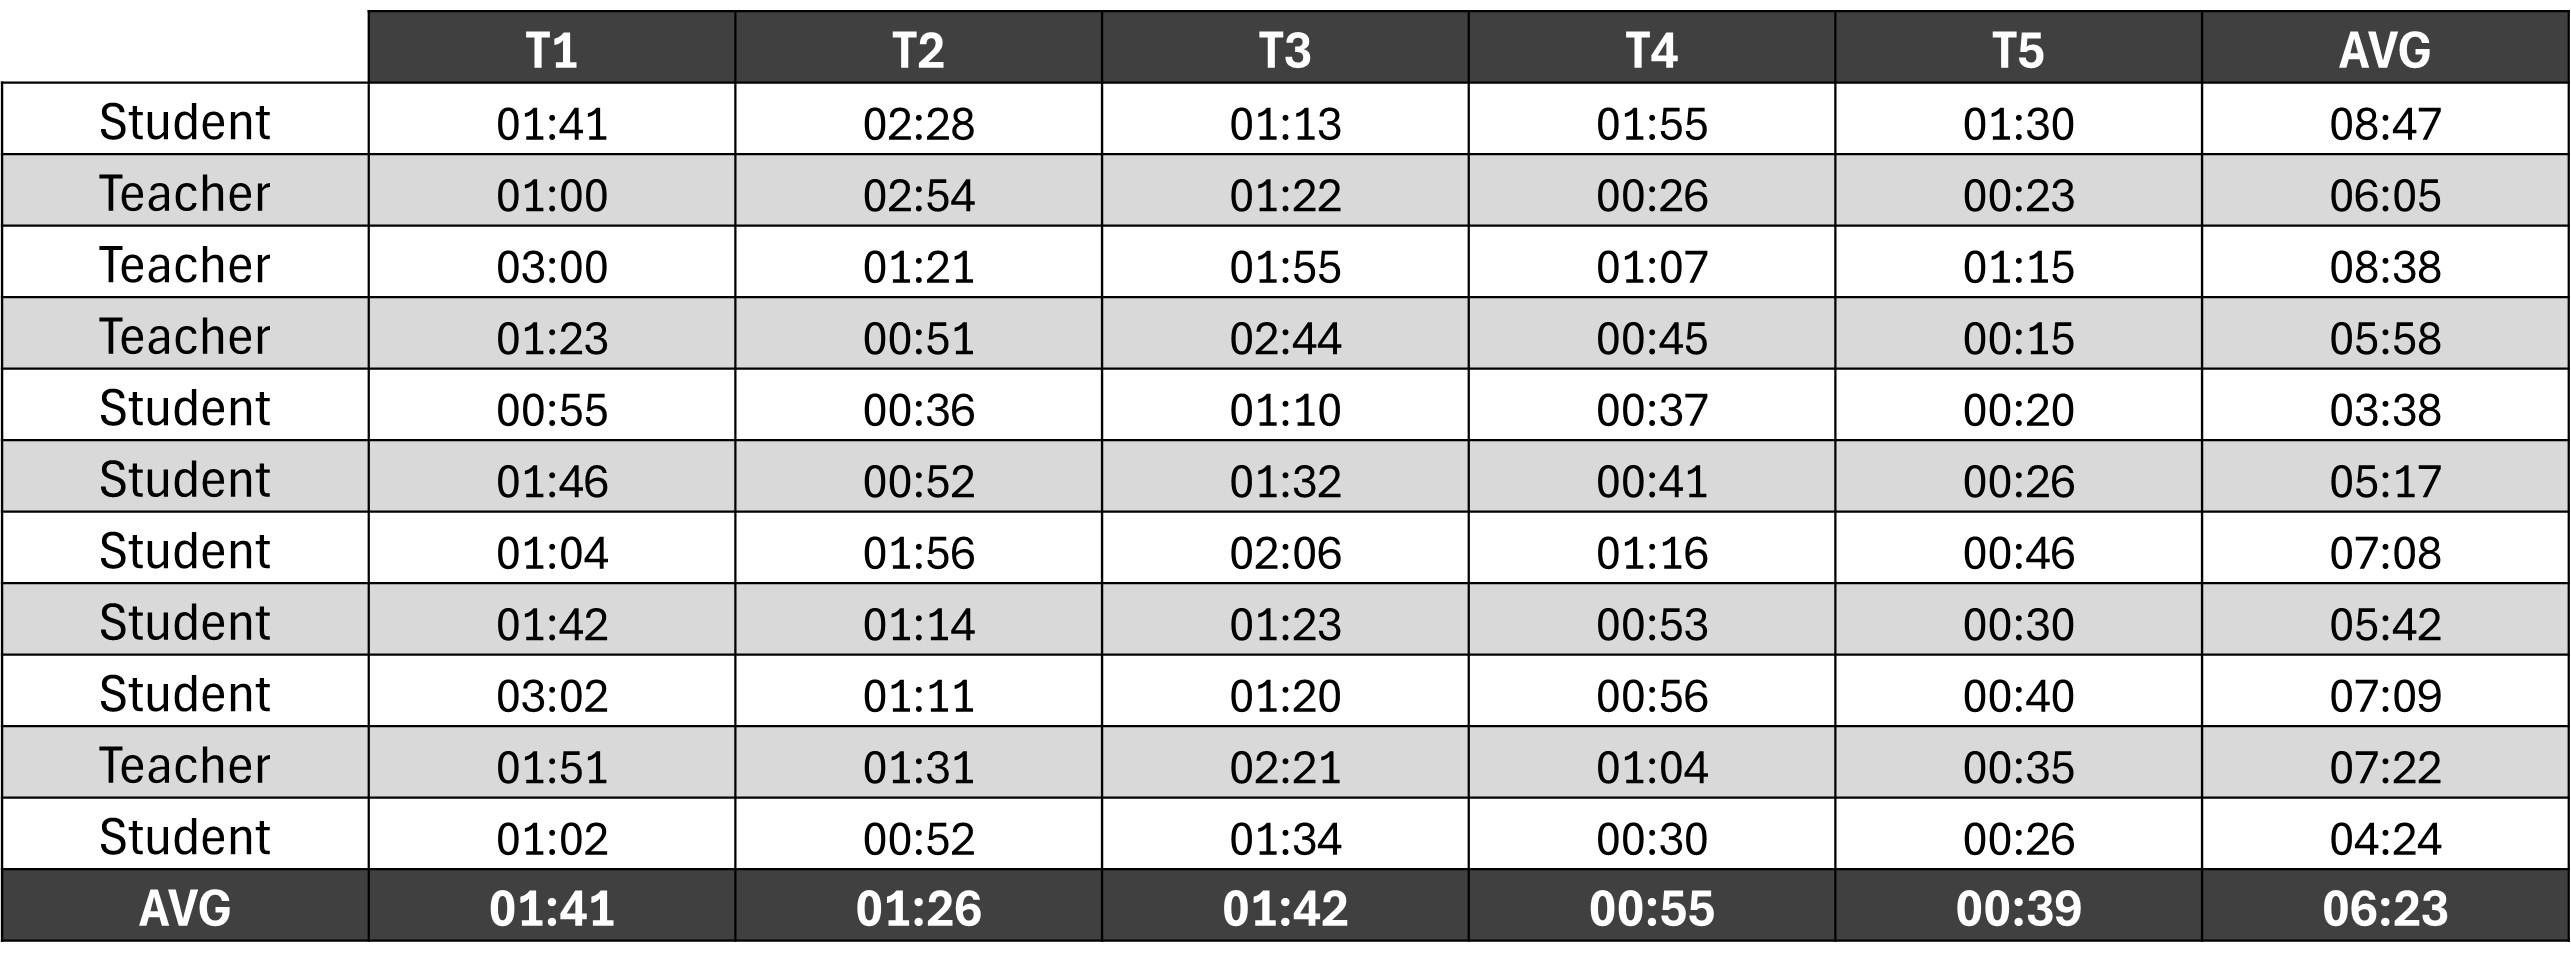
\includegraphics[width=0.95\linewidth]{Chapters/Figures/times.jpg}
    \caption{INSERT.}
    \label{fig:times}
\end{figure}

We noticed that some users struggled with the drag and drop feature, as not being as intuitive as we hope. The way that it worked was by dragging the conclusion of the proof we want to nest inside the other tree, as we noticed that this is very specific and the user need to know that before hand, so based on the observation we understand that instead of grabbing the conclusion it would be more intuitive to drag the whole tree. The other improvement that we collected by observation, was to allow user to append rules to the formulas in both ways, our initial approach pass only by allowing users to apply rules only on top of formulas but whent they start the proof the other way around is more difficult to apply that process as the user as to add first a new empty tree to then apply the rule. There were alot feedback from the users with minor things like some  token replacement values were missing in the formula input box, that some fields could be automatically filled in some rules etc. Every suggestion was take into account and were implemented.

